\begin{tikzpicture}
\node[anchor=north west,inner sep=0] (image) at (0,0) {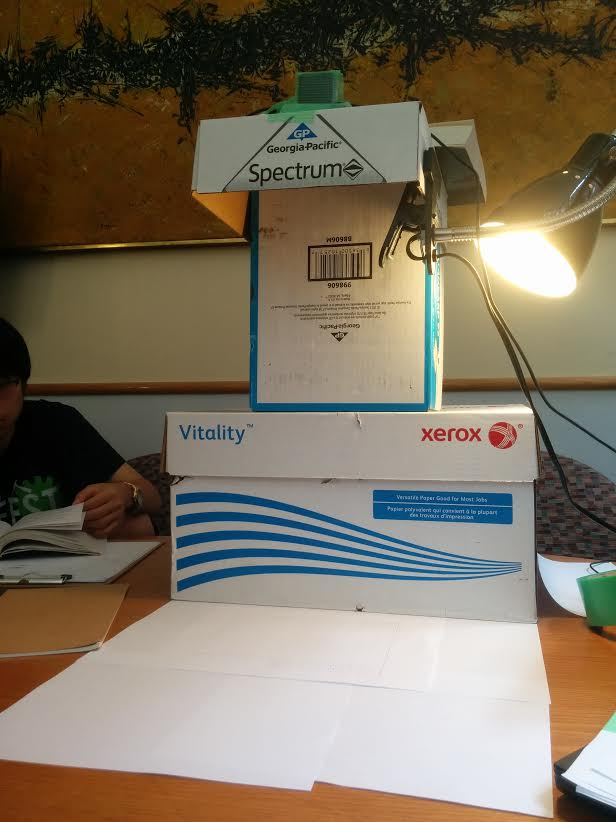
\includegraphics[width=7cm]{device.jpg}};
\begin{scope}[x={7cm / 616},y={-7cm / 616}]
 \draw[red,ultra thick,<-] (350, 90) -- ++(50, 0) node[right,font=\bf\Large] {Camera};
 \draw[red,ultra thick,<-] (520, 320) -- ++(-50, 50) node[below,font=\bf\Large] {Light source};
 \draw[red,ultra thick,<-] (340, 720) node[below,font=\bf\Large] {Paper canvas};
 %\draw[red,ultra thick,<-] (50, 366) -- ++(100, 0) node[right,font=\Large] {A stranger};
\end{scope}
\end{tikzpicture}
